% !TeX root = ../tg.tex

\chapter{低质量数据下SFL的收敛性分析}
\section{引言}
本章旨在从理论层面剖析 non-IID 数据分布与标签噪声对 SFL 收敛性的联合影响。其中的核心难点在于：如何在收敛性分析框架内，精确刻画标签噪声对收敛行为的量化作用。
尽管文献 \cite{ke2023impact} 已在联邦学习领域对标签噪声进行了量化，但其聚焦于模型的泛化能力而非收敛性，故其分析范式无法直接迁移至本场景。据现有文献调研，目前尚无研究在分布式学习算法的收敛性分析中建立标签噪声的量化模型。
针对这一缺失，本章提出一种新的分析路径：首先推导标签噪声对随机梯度的期望的平方与方差的具体扰动，进而将其嵌入传统的收敛性证明框架以推导收敛速率。该策略不仅成功将标签噪声纳入 SFL 的理论分析体系，也为其他分布式学习算法的收敛性研究提供了通用的方法论参考。
在完成理论分析后，本章还通过实验展示了non-IID数据和标签噪声对SFL收敛造成的实际影响。
\section{低质量数据下的SFL框架}
% \subsection{系统模型和问题背景}
% 我们考虑一个包含 $N$ 个客户端的集合，即 $\N=\{1,2,\ldots, N\}$，这些客户端通过SFL协作训练一个全局模型。每个客户端 $n$ 都拥有一个本地数据集 $\Dnoi_n$，由于在数据收集和处理过程中可能存在标签错误和人为误差，该数据集可能包含标签噪声 \cite{lukasik2020does,ji2024fedfixer}。$\Dnoi_n$ 中的每一个数据样本 $i$ 被表示为 $(x_i,\tilde{y}_i)$，其中带有噪声的标签 $\tilde{y}_i$ 可能与真实标签 $y_i$ 不同,并且不同用户间数据的标签分布不一定是独立IID的。

% 为了方便起见，我们为每个客户端 $n$ 定义一个干净的数据集 $\Dcle_n$，它与 $\Dnoi_n$ 相关联，但其中的标签噪声已被修正。$\Dcle_n$ 中的每个数据样本 $i$ 被表示为 $(x_i,y_i)$，其标签噪声已通过数据清晰技术被去除。令 $D_n=|\Dnoi_n|=|\Dcle_n|$ 表示客户端 $n$ 数据集中数据样本的数量。

% 在一个SFL系统中，我们使用 $\omegab$ 来表示全局模型。该全局模型被划分为两个部分：一个 $l_{c}$ 层的客户端模型，记作 $\omegabc$；一个 $l_{s}$ 层的服务器模型，记作 $\omegabs$。特别地，客户端模型 $\omegabc$ 和服务器模型 $\omegabs$ 共同构成完整的全局模型，即 $\omegab = (\omegabc,\omegabs)$。

% 在SFL系统中有两个服务器（如图~\ref{fig:sfl} 所示）：
% \begin{figure}
%     \centering
%     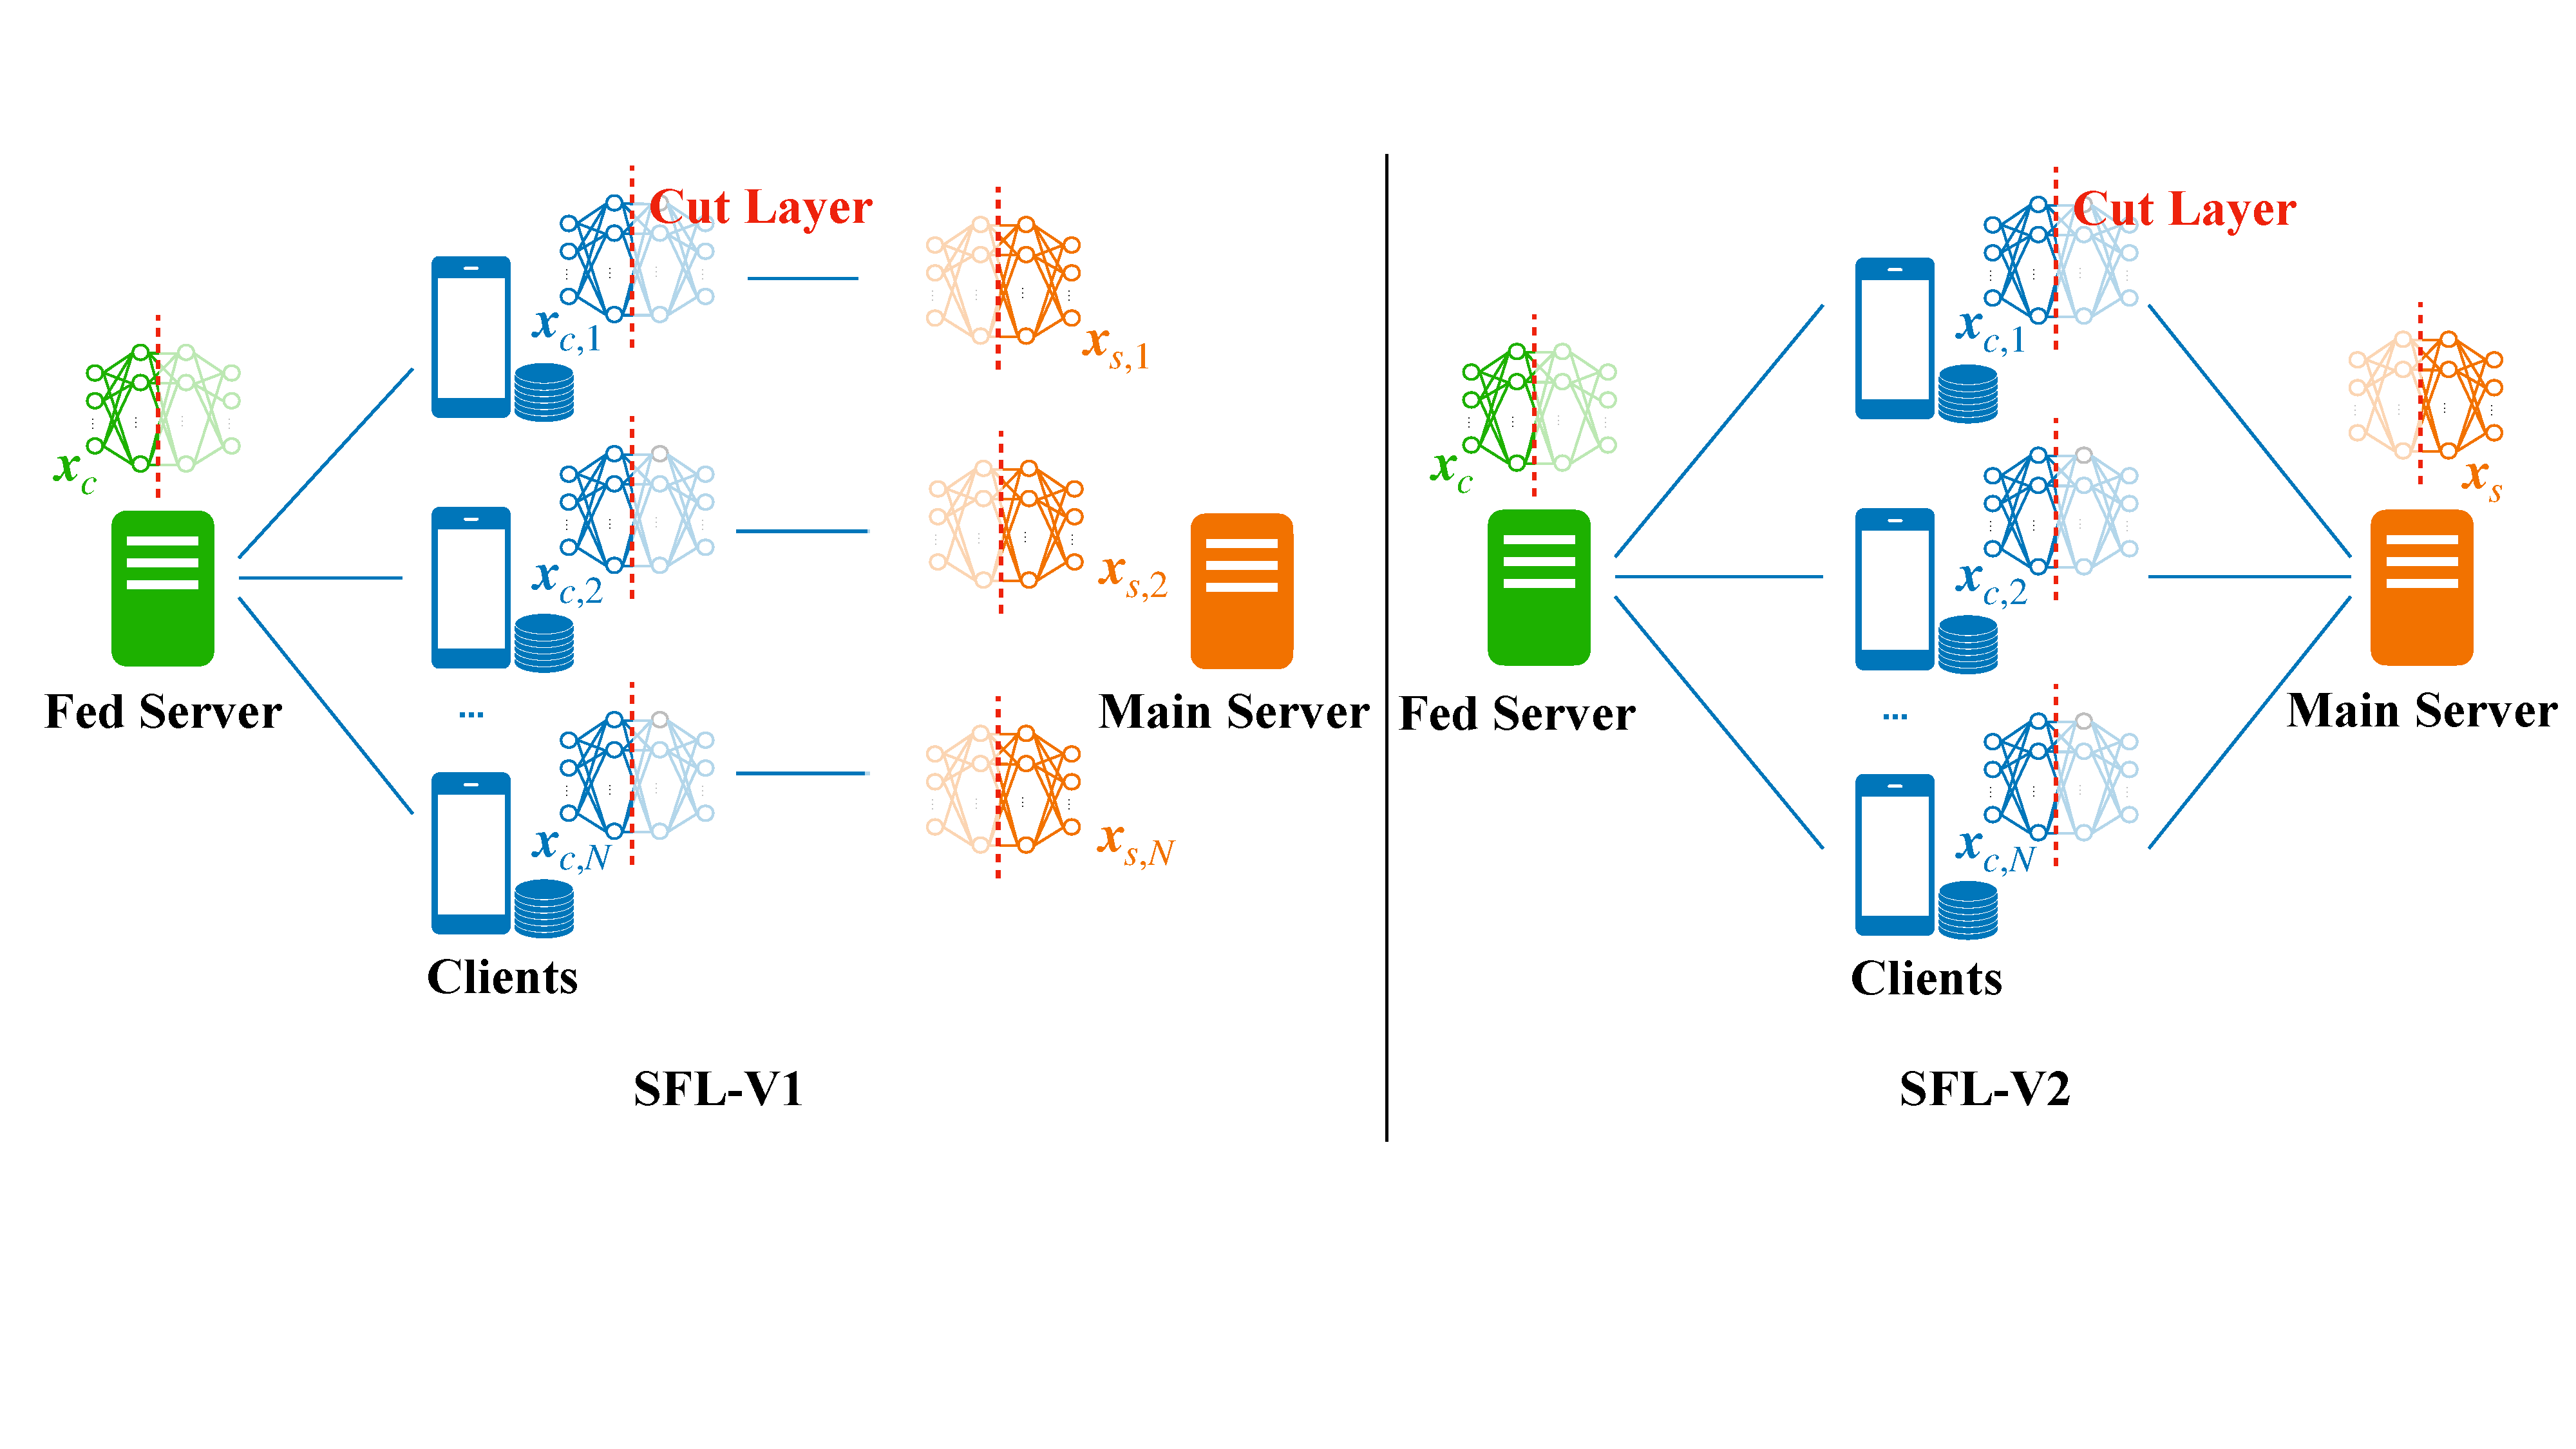
\includegraphics[height=5.6cm]{figures/splitfed.pdf}
%     % \vspace{-6pt}
%     \caption{SFL的两种算法变体：SFL-V1和SFL-V2}
%     \label{fig:sfl}
%     % \vspace{-15pt}
% \end{figure}
    
% \begin{itemize}
%     \item \textbf{联邦服务器}（Fed Server）：负责聚合各客户端上传的模型参数，以生成全局客户端模型 $\omega_c$。
    
%     \item \textbf{训练服务器}（Training Server）：负责执行服务器端模型的训练任务；此外，在涉及多副本服务器模型的场景下，该服务器还负责对分散的服务器端模型进行聚合，从而生成全局服务器端模型 $\omega_s$。
% \end{itemize}

% SFL框架下主要存在两种典型的算法变体：SFL-V1 和 SFL-V2 \cite{thapa2022splitfed}。二者最显著的区别在于训练服务器中模型的更新与维护策略。

% 具体而言，在 SFL-V1 中，训练服务器为每个参与客户端维护一个独立的服务器端模型副本，使得服务器模型与客户端模型之间建立严格的一一映射关系。SFL-V1 的训练流程与FL高度相似，其核心差异在于模型计算负载的分配：FL 要求客户端在本地训练完整模型，而 SFL-V1 将模型划分为客户端模型与服务器端模型，前者在客户端本地训练，后者在训练服务器上训练。此外，SFL-V1 在聚合阶段需同时对客户端模型参数和服务器模型参数进行聚合，以分别构建全局的客户端模型和全局的服务器模型。

% 而在 SFL-V2 中，训练服务器上仅维护一个全局共享的服务器模型。每个客户端在训练时均使用该全局服务器模型与本地客户端模型进行交互。此种架构下，客户端模型更多保留了FL的分布式聚合特征，而服务器模型则体现了SL的集中式训练特征。在模型更新机制上，SFL-V2 仅需对客户端模型进行联邦聚合，训练服务器上的唯一模型作为全局模型直接通过接收到的梯度信息进行更新，无需进行聚合操作。
% \begin{enumerate}
%     \item[(i)] 如文献 \cite{thapa2022splitfed} 所建议，SFL-V2 的性能通常优于 SFL-V1；
%     % \item[(ii)] \rev{SFL-V1 的训练逻辑与 FedAvg 相同，只是部分训练过程被移到了服务器端进行；}
%     \item[(ii)] SFL-V2 的分析比 SFL-V1 更具挑战性。\footnote{我们的分析可以通过遵循现有的联邦学习收敛性分析文献（例如 \cite{b11,karimireddy2020scaffold}）扩展到 SFL-V1。}
% \end{enumerate}
\subsection{问题背景与数学模型}\label{subsec:sfl math back}
我们考虑一个包含 $N$ 个客户端的集合，即 $\mathcal{N}=\{1,2,\ldots, N\}$，
这些客户端通过 SFL 协作训练一个全局模型。每个客户端 $n$ 都拥有一个本地数据集 
$\mathcal{D}^{\text{noi}}_n$，由于在数据收集和处理过程中可能存在标签错误和人为误差，
该数据集可能包含标签噪声 \cite{lukasik2020does,ji2024fedfixer}。
$\mathcal{D}^{\text{noi}}_n$ 中的每一个数据样本 $i$ 被表示为 
$(x_i,\tilde{y}_i)$，其中带有噪声的标签 $\tilde{y}_i$ 可能与真实标签 $y_i$ 不同，
并且不同用户间数据的标签分布不一定是IID的。

为了方便起见，我们为每个客户端 $n$ 定义一个干净的数据集 
$\mathcal{D}^{\text{cle}}_n$，它与 $\mathcal{D}^{\text{noi}}_n$ 相关联，
但其中的标签噪声已被修正。$\mathcal{D}^{\text{cle}}_n$ 中的每个数据样本 $i$ 被表示为
 $(x_i,y_i)$，其标签噪声已通过数据清洗技术被去除。令 $D_n=|\mathcal{D}^{\text{noi}}_n|=|\mathcal{D}^{\text{cle}}_n|$ 
 表示客户端 $n$ 数据集中数据样本的数量。

在一个 SFL 系统中，我们使用 $\boldsymbol{\omega}$ 来表示全局模型。
该全局模型被划分为两个部分：一个 $l_{c}$ 层的客户端模型，
记作 $\boldsymbol{\omega}_c$；
一个 $l_{s}$ 层的服务器模型，记作 $\boldsymbol{\omega}_s$。
特别地，客户端模型 $\boldsymbol{\omega}_c$ 和服务器模型 $\boldsymbol{\omega}_s$ 
共同构成完整的全局模型，即 $\boldsymbol{\omega} = (\boldsymbol{\omega}_c,\boldsymbol{\omega}_s)$。

\subsection{系统架构与算法变体}\label{subsec:sflv1 and v2}
SFL 系统架构中包含两个关键服务器角色（如图~\ref{fig:sfl} 所示），
它们协同工作以支持不同的训练策略：

\begin{figure}[htbp]
    \centering
    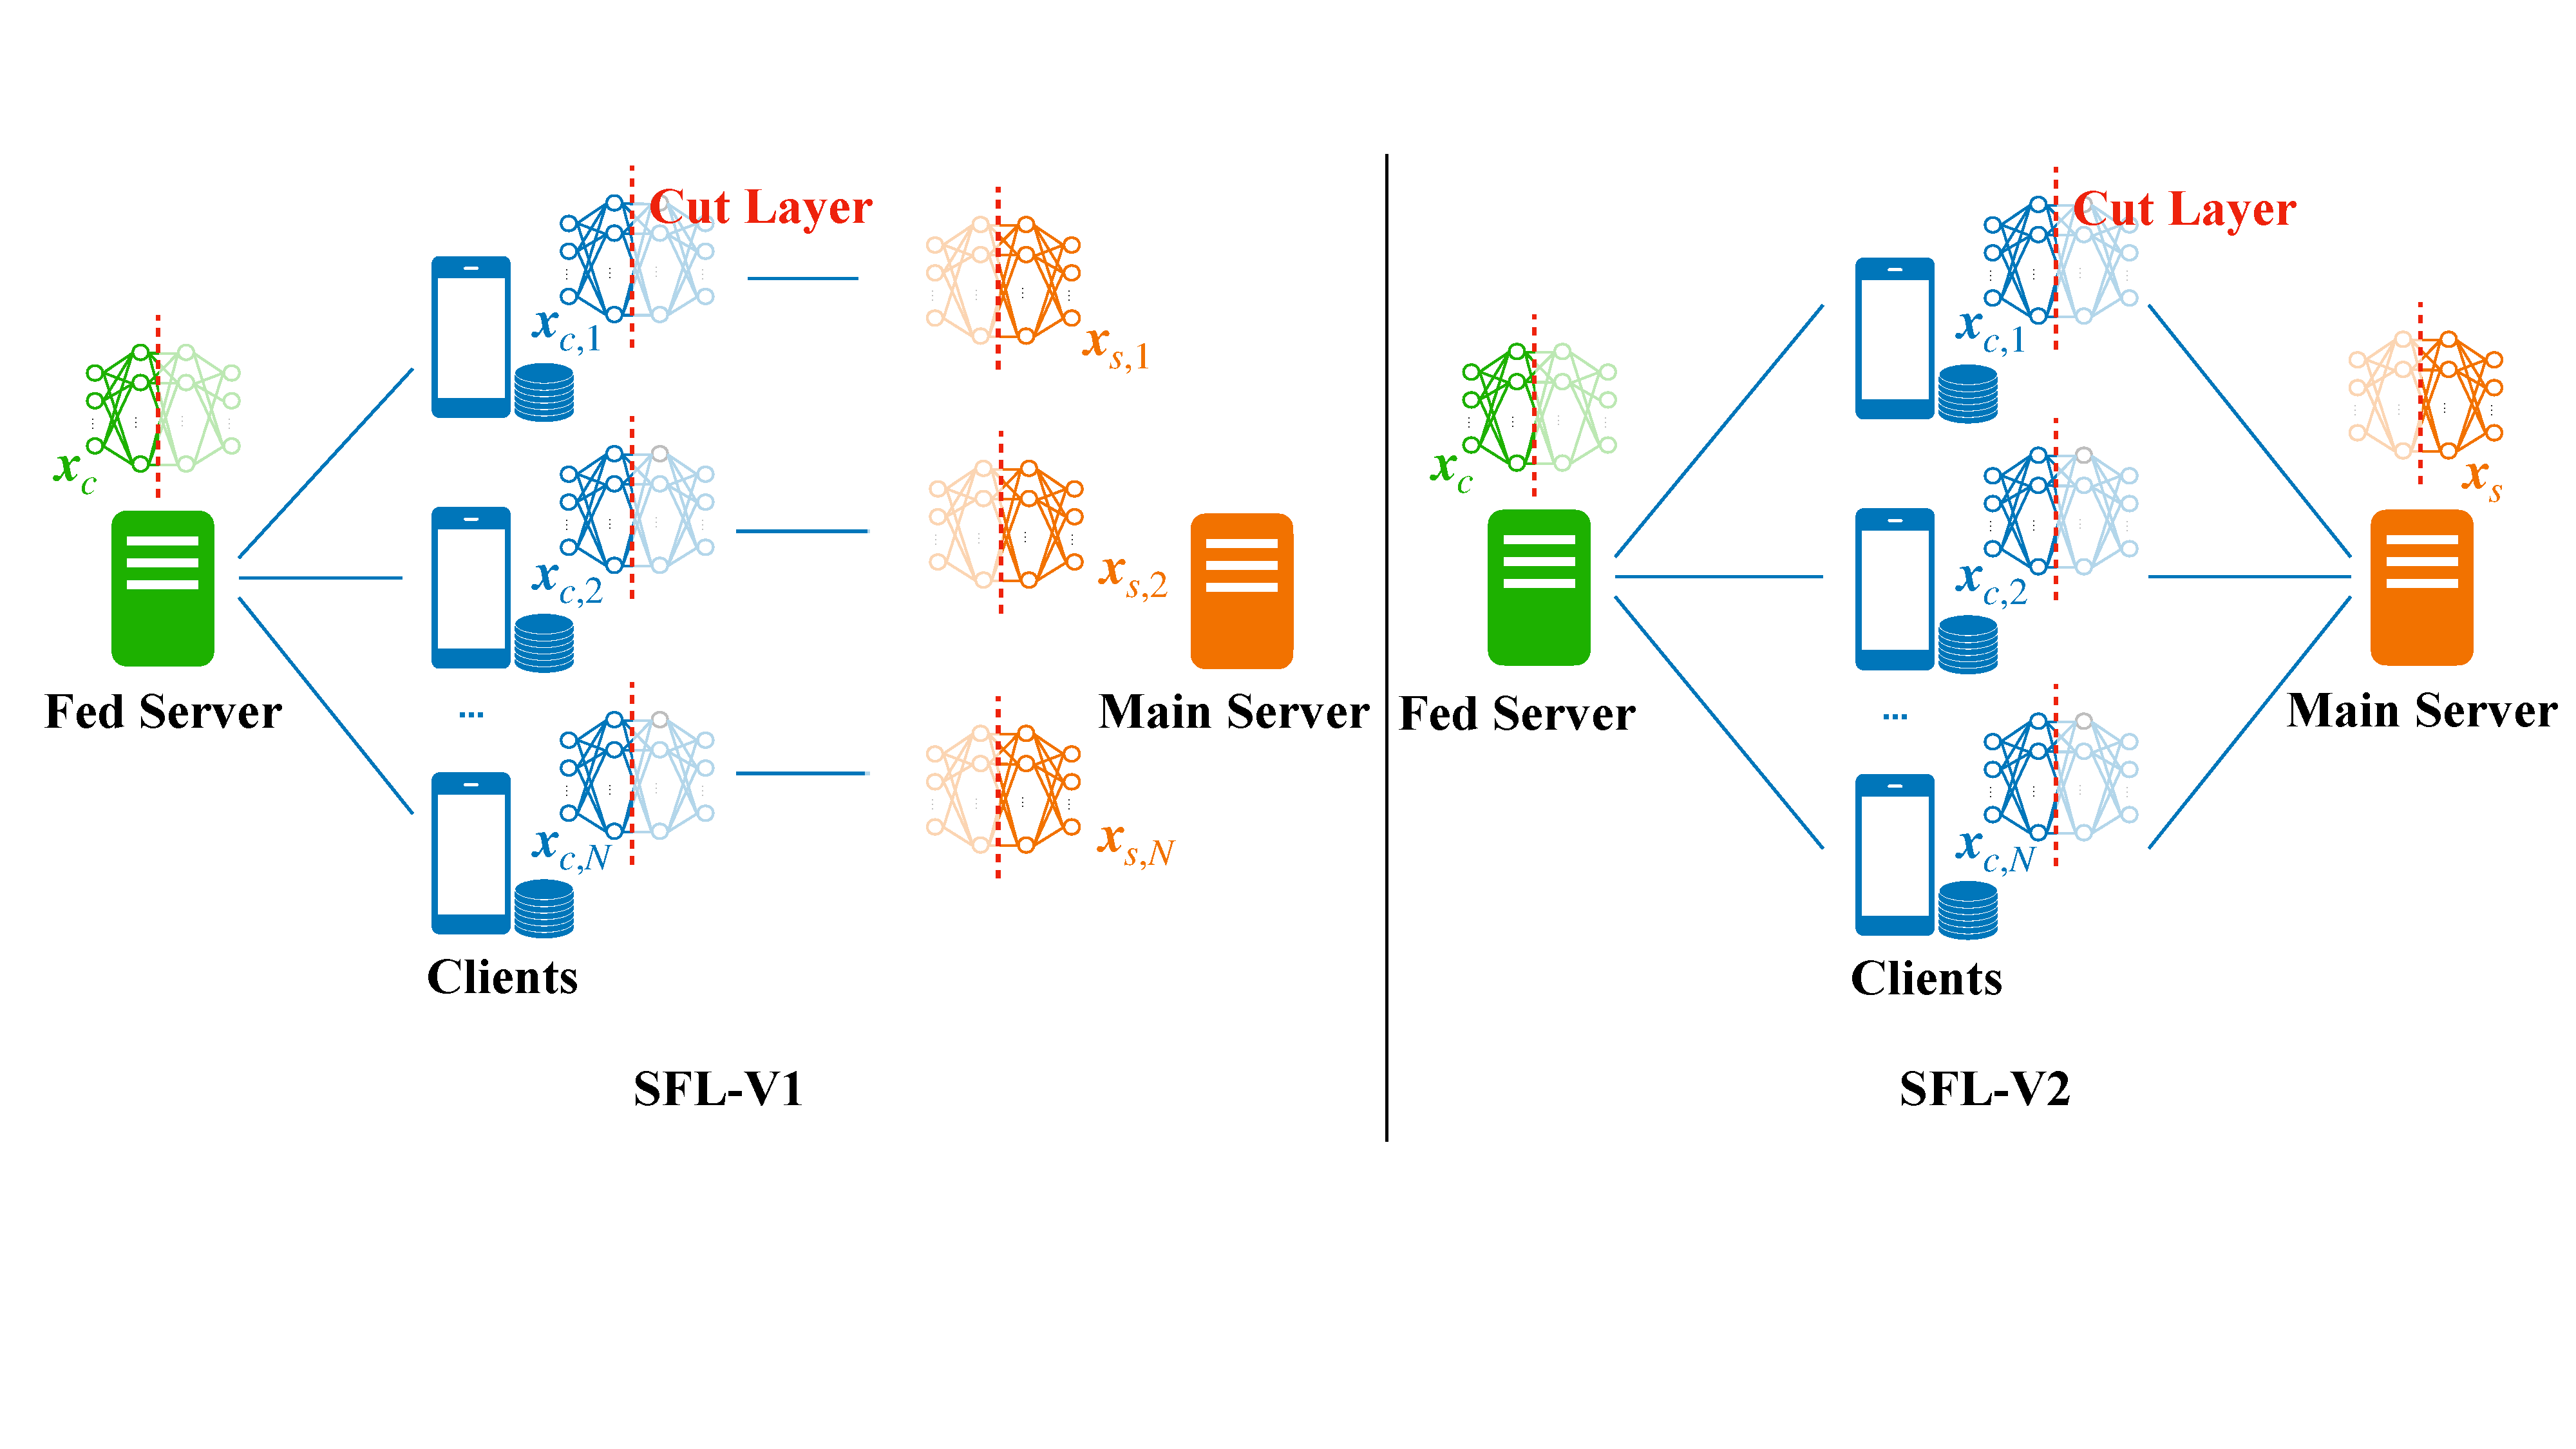
\includegraphics[height=5.6cm]{figures/splitfed.pdf}
    \caption{SFL 的两种算法变体：SFL-V1 和 SFL-V2}
    \label{fig:sfl}
\end{figure}

\begin{itemize}
    \item \textbf{联邦服务器}（Fed Server）：负责聚合各客户端上传的模型参数，以生成全局客户端模型 $\boldsymbol{\omega}_c$。
    
    \item \textbf{训练服务器}（Training Server）：负责执行服务器端模型的训练任务；此外，在涉及多副本服务器模型的场景下，该服务器还负责对分散的服务器端模型进行聚合，从而生成全局服务器端模型 $\boldsymbol{\omega}_s$。
\end{itemize}

基于上述架构，SFL主要存在两种典型的算法变体：SFL-V1 和 SFL-V2 \cite{thapa2022splitfed}。二者最显著的区别在于训练服务器中模型的更新与维护策略。

具体而言，在SFL-V1 中，训练服务器为每个参与训练的客户端维护一个独立的服务器端模型副本，
使得服务器模型与客户端模型之间建立严格的一一映射关系。
SFL-V1 的训练流程与FL高度相似，其核心差异在于模型计算负载的分配：
传统 FL 要求客户端在本地训练完整模型，而 SFL-V1 将模型划分为客户端模型与服务器模型，
前者在客户端本地训练，后者在训练服务器上训练。此外，SFL-V1 在聚合阶段需
同时对客户端模型参数和服务器模型参数进行聚合，以分别构建全局的客户端模型和全局的服务器模型。

而在 SFL-V2 中，训练服务器上仅维护一个全局共享的服务器模型。
每个客户端在训练时均使用该全局服务器模型与本地客户端模型进行交互。
此种架构下，客户端模型更多保留了 FL 的分布式聚合特征，
而服务器模型则体现了SL的集中式训练特征。在模型更新机制上，SFL-V2 
仅需对客户端模型进行聚合，训练服务器上的唯一模型作为全局模型直接通过接收到的梯度信息
进行更新，无需进行额外的聚合操作。
% \subsection{SFL的训练过程}\label{subsec:training}
% SFL的训练持续 $R$ 轮。在每一轮 $r$ 中，客户端 $n \in \mathcal{N}$ 从
% 联邦服务器下载上一轮的全局客户端模型 $\omegabcn^{r-1}$，该模型作为第 $r$ 轮中客户端 $n$ 的
% 初始模型 $\omegabcn^{r}$。  
% 令 $\omegabs^{r}$ 表示第 $r$ 轮的服务器模型，其由上一轮的服务器模型初始化而来。在第 $r$ 轮中，客户端 $n$ 和服务器使用数据集 $\mathcal{D}_{n}^{\text{oi}}$ 对模型进行 $E$ 轮（epoch）的训练。在每一轮中，客户端将其数据集划分为多个小批量（mini-batch），并依次用于对模型 $\omegabcn^{r}$ 和 $\omegabs^r$ 进行更新。第 $r$ 轮中针对一个小批量 $\zetanoi_n \subset \mathcal{D}_{n}^{\text{oi}}$ 的训练过程包含以下四个步骤：

% \textbf{步骤 1：客户端前向传播}。客户端 $n$ 使用小批量 $\zetanoi_n$ 在其本地客户端侧模型 $\omegabcn^{r}$ 上进行前向传播。

% 随后，每个客户端将其计算得到的中间激活值（即 $\omegabcn^{r}$ 前向传播的输出）以及数据标签发送给训练服务器。

% \textbf{步骤 2：训练服务器前向传播}。训练服务器在接收到客户端的中间激活值后，在模型 $\omegabs^{r}$ 上执行前向传播以生成预测标签并计算损失函数。需要注意的是，服务器侧模型 $\omegabs^{r}$ 对某个客户端激活值的更新仅在其之前对其他更早到达的客户端激活值的更新完成后才开始。

% \textbf{步骤 3：训练服务器反向传播}。训练服务器根据计算出的损失函数计算梯度，并据此更新模型 $\omegabs^{r}$。由于服务器侧模型 $\omegabs^{r}$ 仅包含完整模型中的 $l_s$ 层，训练服务器会将中间梯度发送回客户端 $n$，以便其更新客户端侧模型 $\omegabcn$。

% \textbf{步骤 4：客户端反向传播}。客户端 $n$ 在接收到中间梯度后，继续完成反向传播过程，从而更新本地的客户端侧模型 $\omegabcn^r$。至此，一个小批量的训练过程完成。

% \textbf{步骤 5：模型聚合}。  
% 在每一轮训练中，每个客户端 $n$ 需要与训练服务器进行 $E \times \left\lceil \frac{|\mathcal{D}_n|}{|\zeta_n|} \right\rceil$ 次交互，以确保客户端 $n$ 的数据被使用 $E$ 次。当所有客户端完成训练后，联邦服务器通过加权平均的方式计算全局客户端侧模型 $\omegabc^r$：
% \begin{equation}\label{eq:c-agg}
% \omegabc^r=\sum_{n=1}^{N}\frac{|\mathcal{D}_n|}{\sum_{n'=1}^{N}|\mathcal{D}_{n'}|}\omegabcn^r.
% \end{equation}
% 注意，训练服务器维护着全局的服务器侧模型 $\omegabs^r$，无需对其进行聚合操作。  
% 当客户端和服务器完成 $R$ 轮训练后，最终的完整模型为 $\omegab^R=(\omegabc^R,\omegabs^R)$。
\subsection{SFL 的训练过程}\label{subsec:training}
SFL 的训练持续 $R$ 轮。在每一轮 $r$中，训练流程根据具体的算法变体（SFL-V1 或 SFL-V2）略有不同，但总体遵循以下框架：

\textbf{1. 模型初始化与分发}：
在每一轮开始时，客户端 $n \in \mathcal{N}$ 从联邦服务器下载上一轮的全局客户端模型 $\boldsymbol{\omega}_c^{r-1}$，该模型作为第 $r$ 轮中客户端 $n$ 的初始本地模型 $\boldsymbol{\omega}_{c,n}^{r}$。
对于服务器端模型：
\begin{itemize}
    \item 在 SFL-V1 中，训练服务器为每个客户端 $n$ 维护一个独立的服务器模型副本 $\boldsymbol{\omega}_{s,n}^{r}$，这些副本由上一轮聚合后的全局服务器模型 $\boldsymbol{\omega}_s^{r-1}$ 初始化。
    \item 在 SFL-V2 中，训练服务器仅维护一个全局共享的服务器模型 $\boldsymbol{\omega}_s^{r}$，该模型由上一轮的 $\boldsymbol{\omega}_s^{r-1}$ 直接继承。
\end{itemize}

\textbf{2. 客户端与服务器协同训练}：
在第 $r$ 轮中，每个客户端 $n$ 使用其本地数据集 $\mathcal{D}_{n}^{\text{noi}}$ 对模型进行 $E$ 个 epoch（即所有训练样本被完整遍历一次的轮次） 的训练。在每个 epoch 中，客户端将数据划分为多个小批量（mini-batch），记为 $\zeta_n \subset \mathcal{D}_{n}^{\text{noi}}$，并依次执行以下四个步骤来完成一个mini-batch的更新：

\begin{description}
    \item[步骤 1：客户端前向传播] 
    客户端 $n$ 使用小批量 $\zeta_n^{noi}$ 在其本地模型 $\boldsymbol{\omega}_{c,n}^{r}$ 上进行前向传播，计算出中间激活值（即切分层的输出）。随后，客户端将这些中间激活值以及对应的标签发送给训练服务器。

    \item[步骤 2：训练服务器前向传播] 
    训练服务器接收到中间激活值后，利用当前的服务器端模型（在 V1 中为对应的副本 $\boldsymbol{\omega}_{s,n}^{r}$，在 V2 中为全局模型 $\boldsymbol{\omega}_s^{r}$）执行前向传播，生成预测结果并计算损失函数。

    \item[步骤 3：训练服务器反向传播] 
    训练服务器根据损失函数计算梯度，并更新相应的服务器端模型参数。由于服务器端模型仅包含完整模型的后 $l_s$ 层，训练服务器会将关于中间激活值的梯度（即“切分层梯度”）发送回客户端 $n$。

    \item[步骤 4：客户端反向传播] 
    客户端 $n$ 接收到梯度后，结合本地保存的前向传播信息，继续完成剩余层的反向传播过程，从而更新本地的客户端模型 $\boldsymbol{\omega}_{c,n}^{r}$。至此，一个小批量的训练迭代完成。
\end{description}

% 上述过程重复进行，直到每个客户端完成 $E$ 个 epoch 的训练，即每个客户端与训练服务器共进行 $E \times \left\lceil \frac{|\mathcal{D}_n|}{|\zeta_n|} \right\rceil$ 次交互。

\textbf{3. 模型聚合}：
SFL-V1和SFL-V2的客户端模型聚合频率
均为$\kappa=\left\lceil \frac{D_n}{b} \right\rceil \times E$，SFL-V1服务器
模型的聚合频率为$\tilde{\kappa}$,其中$\tilde{\kappa}$与$\kappa$不一定相等。
聚合阶段的具体操作取决于 SFL 的具体变体，其过程入戏：
\begin{itemize}
    \item \textbf{客户端模型聚合}：无论何种变体，联邦服务器都会收集所有客户端上传的 $\boldsymbol{\omega}_{c,n}^{r}$，并通过加权平均生成新一轮的全局客户端模型 $\boldsymbol{\omega}_c^r$：
    \begin{equation}\label{eq:c-agg}
    \boldsymbol{\omega}_c^r=\sum_{n=1}^{N}\frac{|\mathcal{D}_n|}{\sum_{n'=1}^{N}|\mathcal{D}_{n'}|}\boldsymbol{\omega}_{c,n}^r.
    \end{equation}

    \item \textbf{服务器模型处理}：
    \begin{enumerate}
        \item \textbf{SFL-V1}：训练服务器对各客户端对应的服务器模型副本执行与公式\ref{eq:c-agg}中类似的加权平均操作，生成全局服务器模型 $\boldsymbol{\omega}_s^r$，用于初始化下一轮的各个副本。
        \item \textbf{SFL-V2}：由于训练服务器上的全局模型 $\boldsymbol{\omega}_s^{r}$ 已经在步骤 3 中通过接收到的梯度进行了实时累积更新，因此无需额外的聚合操作。当前的 $\boldsymbol{\omega}_s^{r}$ 直接作为本轮的全局服务器模型进入下一轮。
    \end{enumerate}
\end{itemize}

当客户端和服务器完成 $R$ 轮训练后，最终的完整全局模型由聚合后的客户端部分和服务器部分组成，即 $\boldsymbol{\omega}^R=(\boldsymbol{\omega}_c^R,\boldsymbol{\omega}_s^R)$。
\subsection{分割-联邦学习的训练目标}

% 具体而言，令 $\zetacle_n$ 表示客户端 $n$ 的干净数据集 $\Dcle_n$ 中的一个小批量。令 $F_n(\omegab;\zetacle_n)$ 表示完整模型 $\omegab$ 在客户端 $n$ 的小批量 $\zetacle_n$ 上的损失函数。客户端 $n$ 的期望损失由下式给出：
% \begin{equation}\label{eq:exp-fn}
% \fcle_n\left(\omegab\right)=\mathbb{E}_{\zetacle_n\sim \Dcle_n}\left[F_n\left(\omegab;\zetacle_n\right)\right].
% \end{equation}
% SFL 的目标是学习一个模型 $\omegab^*$，以最小化所有客户端之间 $F_{n}(\omegab)$ 的加权平均~\cite{b8}：
% \begin{equation}\label{Objective of SFL}
% \omega^* = \arg\min_{\omega} \sum_{n=1}^{N} \frac{|\mathcal{D}_n|}{\sum_{n'=1}^{N} |\mathcal{D}_{n'}|} \, F^{\mathrm{cle}}_{n}(\omega).
% \end{equation}
% 需要注意的是，SFL 训练过程是基于所有 $n\in\N$ 的含噪数据集 $\Dnoi_n$ 执行的；然而，如公式 (\ref{Objective of SFL}) 所述，其目标在于使模型 $\omegab^R$ 拟合所有 $n\in\N$ 的干净数据集 $\Dcle_n$。下文首先分析 $\Dnoi_n$ 与 $\Dcle_n$ 之间的上述差异如何降低 SFL 的收敛速率。随后，我们提出一种算法以缓解标签噪声带来的影响。
具体而言，令 $\zetacle_n$ 表示客户端 $n$ 的干净数据集 $\Dcle_n$ 中的一个小批量。设 $F_n(\omegab;\zetacle_n)$ 表示完整模型 $\omegab$ 在客户端 $n$ 的小批量 $\zetacle_n$ 上的损失函数。客户端 $n$ 的期望损失为  
\begin{equation}\label{eq:exp-fn}
\fcle_n\left(\omegab\right)=\mathbb{E}_{\zetacle_n\sim \Dcle_n}\left[F_n\left(\omegab;\zetacle_n\right)\right].
\end{equation}

SFL的目标是学习一个模型 $\omegab^*$，使其最小化所有客户端上损失函数 $F_{n}(\omegab)$ 的加权平均值 \cite{b8}：
\begin{equation}\label{Objective of SFL}
\omegab^* =\arg \min_{\omegab}f(\omegab)\triangleq \sum_{n=1}^{N}\frac{|\D_n|}{\sum_{n'=1}^{N}|\D_{n'}|}F^{cle}_{n}(\omegab).
\end{equation}

值得注意的是，尽管第 \ref{subsec:sfl math back} 至 \ref{subsec:training} 节中描述的 SFL 训练过程是在所有客户端 $n\in\mathcal{N}$ 的含噪数据集 $\mathcal{D}^{\text{noi}}_n$ 上执行的，但其优化目标仍遵循公式 (\ref{Objective of SFL}) 的定义，即令模型 $\boldsymbol{\omega}^R$ 拟合所有客户端的纯净数据集 $\mathcal{D}^{\text{cle}}_n$。

% 接下来，我们将在non-IID数据和标签噪声存在的环境下，分别针对均方误差（MSE）损失函数与交叉熵（Cross-Entropy）损失函数对SFL的收敛性进行分析。
% 随后，我们在第三章提出一种算法以缓解non-IID数据和标签噪声带来的影响。

\section{收敛性理论推导}
本章首先阐述收敛性证明所需的一般假设条件，随后针对均方误差（MSE）与交叉熵（Cross-Entropy）两种损失函数分别进行推导，最后给出相应的收敛性结论。
\subsection{假设条件}
如同许多已有工作（例如 \cite{b4,b11,b8}），本章在收敛分析中对随机梯度和损失函数做出一些假设。令 $\gb_n\left(\omegab,\zeta_n\right)$ 表示 $F_n\left(\omegab;\zeta_n\right)$ 在小批量 $\zeta_n$ 上的随机梯度，即 $\gb_n\left(\omegab,\zeta_n\right)\triangleq \nabla F_n\left(\omegab;\zeta_n\right)$。令 $\nabla \fcle_n(\omegab)$ 表示客户端 $n\in\N$ 的干净数据集上期望损失 $\fcle_n(\omegab)$ 的梯度，定义见公式 \eqref{eq:exp-fn}。令 $\nabla \fnoi_n(\omegab)$ 表示对应于噪声数据集的期望损失梯度。对于任意客户端 $n\in\N$，来自干净数据集 $\Dcle_n$ 的小批量上的随机梯度满足以下假设：

\begin{assumption}[均方误差下随机梯度的方差]\label{ass:gradient-variance}
对于任意客户端 $n\in\N$，$\gb_n\left(\omegab,\zetacle_n\right)$ 在干净小批量上的期望方差是有界的，即：
\begin{equation}\label{eq:gradient-variance}
    \mathbb{E}_{\zetacle_n\sim \Dcle_n}\left[\left\Vert \gb_n\left(\omegab,\zetacle_n\right) - \nabla \fcle_n\left(\omegab\right) \right\Vert^2 \right] \leq \phi_n^2.
\end{equation}
\end{assumption}

\begin{assumption}[均方误差下的随机梯度]\label{ass:gradient}
对于任意客户端 $n\in\N$，$\gb_n\left(\omegab,\zetacle_n\right)$ 在 clean 数据集 $\Dcle_n$ 上的期望随机梯度是有界的，即：
\begin{equation}\label{eq:gradient}
\mathbb{E}_{\zetacle_n\sim \mathcal{D}_n^{cle}}\left[\left\Vert \gb_n\left(\omegab, \zetacle_n\right) \right\Vert^2\right] \leq G_n^2.
\end{equation}
\end{assumption}

\begin{assumption}[数据异构性]\label{ass:heter}
所有客户端 $n\in\N$ 的期望梯度 $\nabla \f_n(\boldsymbol{\omega})$ 的方差是有界的，即：
\begin{equation}
\textstyle \left\Vert 
\nabla \f_n\left(\boldsymbol{\omega}\right)- \sum_{n\in\N}
\nabla\f_n(\boldsymbol{\omega})/N \right\Vert^2 \le \lambda^2.
\end{equation}
这里，$\nabla \f_n(\boldsymbol{\omega})$ 同时表示 $\nabla \f_n^{cle}(\boldsymbol{\omega})$ 和 $\nabla \f_n^{noi}(\boldsymbol{\omega})$。\footnote{注意，non-IID数据和标签噪声可以建模为相互独立的事件，前者涉及客户端的数据分布，后者涉及标签如何被破坏。}
\end{assumption}

\noindent 此外，本文对损失函数作出如下假设：%\footnote{虽然本文使用MSE和Cross-Entorpy作为损失函数，但损失函数相对于全局模型的性质依赖于分割-联邦学习中的模型结构和小批量中的数据样本。因此，如同现有工作（例如 \cite{b4,b11,b8}），我们需要对损失函数施加假设以便进行分析。}

\begin{assumption}[$S$-平滑性]\label{ass:smooth}
对于任意模型 $\omegab_1, \omegab_2\in \mathbb{R}^d$，损失函数是 $S$-平滑的，即：
$$
F_n(\omegab_2) \leq F_n(\omegab_1)+\langle \nabla F_n(\omegab_1), \omegab_2-\omegab_1\rangle +\frac{S}{2}\|\omegab_2-\omegab_1\|^2.
$$
\end{assumption}
为了处理SFL中的模型拆分操作，本文提出以下引理，将期望损失的界分解为两个项，分别对应服务器端和客户端模型。令 $\omegab^*\triangleq(\omegabc^*; \omegabs^*)$ 表示使 $f(\omegab)$ 最小化的最优全局模型，定义见 \eqref{Objective of SFL}。令 $\omegab^R\triangleq(\omegabc^R; \omegabs^R)$ 表示经过 $R$ 轮训练后获得的全局模型。

\begin{lemma}[收敛性分析中的模型拆分 \cite{b8}]\label{lemma:decomp}
通过SFL训练得到的模型与最优模型之间的性能差距上界如下：
\begin{equation}
\mathbb{E}\left[f(\omegab^{R})\right]- f(\omegab^*)\le\frac{S}{2}\left(\mathbb{E}||\omegabs^{R}-\omegabs^*||^2+\mathbb{E}||\omegabc^{R}-\omegabc^*||^2\right).
\end{equation}
\end{lemma}
该引理的证明在附录\ref{app:lemma1}
\subsection{MSE作为损失函数时的收敛性}\label{subsec:mse}
本节深入探讨MSE作为损失函数的设定下，SFL 框架中模型的收敛性质。
MSE 是回归任务中最基础且广泛使用的损失度量。为了从概率视角对标签噪声进行建模，我们假设其服从高斯分布。
具体而言，针对连续值标签 $y_i$，我们引入一个加性随机噪声项 $\epsilon_i$ 来模拟现实场景中的数据不确定性。
形式上，我们将观测到的含噪标签 $\tilde{y}_i$ 建模为真实标签 $y_i$ 与噪声 $\epsilon_i$ 的和：
\begin{equation}
    \tilde{y}_i = y_i + \epsilon_i,
\end{equation}
其中，噪声项 $\epsilon_i$ 服从均值为 $\mu$、方差为 $\sigma^2$ 的正态分布，即 $\epsilon_i \sim \mathcal{N}(\mu, \sigma^2)$。为了保证估计的无偏性，即确保引入噪声后标签的期望值保持不变，我们设定噪声均值 $\mu = 0$。在此假设下，含噪数据集可表示为 $\mathcal{D}_{\text{noi}} = \{(x_i, \tilde{y}_i)\}_{i=1}^N$。
% 在该概率框架下，最小化 MSE 损失函数等价于在独立同分布的高斯噪声假设下最大化数据的对数似然函数。
这种基于加性高斯噪声的建模范式已被现有文献广泛采纳，并为分析深度学习模型在噪声环境下的鲁棒性与收敛行为提供了坚实的理论基础~\cite{frenay2013classification}。
 
\subsubsection{标签噪声对损失函数的影响}
令 $h(x_i; \boldsymbol{\omega})$ 表示由参数向量 $\boldsymbol{\omega}$ 确定的模型对输入特征 $x_i$ 的预测输出，模型 $\omegab$ 在一个无噪声mini-batch $\zeta_n^{cle}$ 上的 MSE 损失函数 $F_{n}(\omegab;\zeta_n^{cle})$ 定义如下：
\begin{equation}\label{eq:mse}
% F_n\left(\omegab;\zeta\right)=\frac{1}{|\zeta|}\sum_{\left(x_i,{y}_i\right)\in \zeta}\left(h\left(x_i;\omegab\right)-{y}_i\right)^2.
F_n\left(\boldsymbol{\omega};\zeta_n^{cle}\right)=\frac{1}{|\zeta_n^{cle}|}\sum_{\left(x_j,y_j\right)\in \zeta_n^{cle}}\left(h\left(x_j;\boldsymbol{\omega}\right)-y_j\right)^2
\end{equation}

\noindent 因此，我们可以将含噪声数据集下的损失函数用干净数据集下的损失函数表示如下：

\begin{lemma}[带标签噪声的MSE]\label{lem:mse}
考虑一个小批量 $\zetanoi_n$ 及其对应的干净小批量 $\zetacle_n$，则有
\begin{multline}
F_n\left(\omegab;\zetanoi_n\right)=F_n\left(\omegab;\zetacle_n\right)
    +\frac{1}{|\zetanoi_n|}\sum_{\left(x_i,\tilde{y}_i\right)\in \zetanoi_n}\left( \epsilon_i^2 - 2\left(h\left(x_i;\omegab\right)-y_i\right)\epsilon_i \right).
\end{multline}
\end{lemma}
\noindent 该引理的证明在附录\ref{app:lemma2}


\subsubsection{标签噪声对梯度的影响}\label{subsubsec:mse gradient}
本节旨在分析标签噪声对随机梯度的影响。
在公式\eqref{eq:gradient-variance}与\eqref{eq:gradient}所定义的随机梯度上界基础上，
本节将推导其在标签噪声场景下的新上界。
% 中定义的与随机梯度相关的新的上界。
在干净数据集上随机梯度$\boldsymbol{g}_n\left(\boldsymbol{\omega},\zeta_n^{cle}\right)$可以表示为：
\begin{equation}\label{Gradient of clean loss}
% \begin{aligned}
\boldsymbol{g}_n\left(\boldsymbol{\omega},\zeta_n^{cle}\right)=\nabla_\omega  F_n\left(\boldsymbol{\omega};\zeta_n^{cle}\right)
=\frac{1}{|\zeta_n^{cle}|}\sum_{\left(x_j,y_j\right)\in \zeta_n^{cle}} \nabla_\omega \left(h\left(x_j;\boldsymbol{\omega}\right)-\left(y_j\right)\right)^2
% \end{aligned}
\end{equation}

在此基础之上，我们可以得到在噪声数据集上的随机梯度 $\gb_n(\omegab,\zetanoi_n)$ 与干净数据集上的随机梯度 $\gb_n(\omegab,\zetacle_n)$ 的关系：
\begin{lemma}[标签噪声下MSE的随机梯度]\label{lem:msegra}
    \begin{multline}\label{Gradient of clean loss}
\gb_n\left(\omegab,\zetanoi_n\right) %= \nabla F_n\left(\boldsymbol{\omega};\zetanoi_n\right)\\
=\gb_n\left(\omegab,\zetacle_n\right)
-\frac{1}{|\zetanoi_n|}\sum_{\left(x_i,y_i+\epsilon_i\right)\in \zetanoi_n}2\epsilon_i \nabla h\left(x_i;\boldsymbol{\omega}\right).
\end{multline}
\end{lemma}

\noindent 该引理的证明在附录\ref{app:lemma3}

基于此，我们给出如下两个命题，它们分别界定了含噪声数据集下的随机梯度的方差和期望的平方。

\begin{proposition}[均方差损失下含标签噪声的随机梯度的方差]\label{prop:variance-g mse}
在假设 \ref{ass:gradient-variance} 下，任意客户端 $n\in\N$ 在噪声小批量上的 $\gb_n\left(\omegab,\zetanoi_n\right)$ 的期望方差是有界的：
\begin{equation}\label{bounded-variance with noise}
     \mathbb{E}_{\zetanoi_n\sim \Dnoi_n}\left[\left\Vert \gb_n\left(\boldsymbol{\omega},\zetanoi_n\right) - \nabla \fnoi_n\left(\boldsymbol{\omega}\right) \right\Vert^2 \right] \leq \phi_n^2+H_1^2,
\end{equation}
其中 $H_1^2$ 定义为：
\begin{align}\label{eq:H}
    H_1^2 &= \frac{8\sigma^2}{|\mathcal{D}_n^{noi}|^2}\sum_{\left(x_{i},y_{i}+\epsilon_{i}\right)\in \mathcal{D}_n^{noi}}\left(
\nabla_\omega  h\left(x_{i};\boldsymbol{\omega}\right)\right)^2 \notag\\
    &+\frac{4\sigma^2}{|\mathcal{D}_n^{noi}||\zeta_n^{noi}|}\sum_{\left(x_{i},y_{i}+\epsilon_{i}\right)\in \mathcal{D}_n^{noi}}\left(
\nabla_\omega  h\left(x_{i};\boldsymbol{\omega}\right)\right)^2
\end{align}
\end{proposition}

\begin{proposition}[均方差损失下含标签噪声的随机梯度的平方的期望]\label{prp:square-g mse}
在假设 \ref{ass:gradient} 下，任意客户端 $n\in\N$ 在噪声数据集 $\Dnoi_n$ 上的 $\gb_n\left(\omegab,\zetanoi_n\right)$ 是有界的，即：
\begin{equation}
    \mathbb{E}_{\zetanoi_n\sim \Dnoi_n}\left[\left\Vert \gb_n\left(\omegab, \zetanoi_n\right) \right\Vert^2\right] \leq G_n^2 + H_2^2,
\end{equation}
其中 $H_2^2$ 定义为：
\begin{align}\label{eq:H}
    H_2^2 &= \sum_{\zeta_n^{noi}\subset\mathcal{D}_n^{noi}} \frac{4\sigma^2}{|\mathcal{D}_n^{noi}||\zeta_n^{noi}|}\sum_{\left(x_{j},y_{j}+\epsilon_{j}\right)\in \zeta_n^{noi}}\left(
\nabla_\omega  h\left(x_{j};\boldsymbol{\omega}\right)\right)^2
\end{align}
\end{proposition}

\noindent 命题~\ref{prop:variance-g mse}和~\ref{prp:square-g mse} 的证明分别见附录~\ref{app:pro1}和~\ref{app:pro2}。

\subsubsection{收敛性结果}\label{proofC}



然后，我们可以得出使用MSE损失函数时关于含噪声数据集的SFL收敛性的主要结果。此处沿用了 \cite{b8} 的证明路径，由于篇幅限制，省略了详细证明。此处我们定义 $b$ 表示mini-batch的尺寸，$\eta^r$表示第$r$轮的学习率,以及：
$$
\kappa_{min}= min\{\kappa,\tilde{\kappa}]\}, \quad\kappa_{max}= max\{\kappa,\tilde{\kappa}\}, \quad a_n= \frac{D_n}{\sum_{n'=1}^{N}D_{n'}}, \quad \forall n.
$$

\noindent 收敛性结果如下，包括SFL-V1和SFL-V2

\begin{theorem}{SFL-V1的收敛性（MSE损失函数）}\label{theorem-v1-full-mse}
 % Let Assumptions \ref{assump: smoothness}-\ref{assump: heterogeneity} hold. 
 % {\color{red}Assumption \ref{assump: heterogeneity} is not used?}

\noindent \textbf{一般凸情形：}:  在假设 \ref{ass:gradient-variance}--\ref{ass:smooth} 以及均方差损失函数下，若 $\eta^r \leq \frac{1}{2 S\kappa}$, 

\begin{equation}\label{bound-v1-gc-full}
\begin{aligned}
\mathbb{E}\left[f\left(\boldsymbol{\omegab}^{R}\right)\right]-f^*\le &\frac{S\left\|\boldsymbol{\omegab}^{0}-\boldsymbol{\omegab}^{\ast}\right\|^2}{2(R+1)}\\ 
&+ O\left(\left(\frac{(\kappa^2+\tilde{\kappa})^2\left\|\boldsymbol{\omegab}^{0}-\boldsymbol{\omegab}^{\ast}\right\|^2 N}{\kappa_{min}^2(R+1)}\sum_{n=1}^Na_n^2\left(\sigma_n^2+G^2+H_1^2+H_2^2\right)\right)^{\frac{1}{2}}\right)\\
    &+O\left(\left(\frac{(\kappa^2+\tilde{\kappa})^2S \left\|\boldsymbol{\omegab}^{0}-\boldsymbol{\omegab}^{\ast}\right\|^2}{\kappa_{min}^2(R+1)}\sum_{n=1}^Na_n\left(\sigma_n^2+G^2+H_1^2+H_2^2\right)\right)^{\frac{1}{3}}\right).
\end{aligned}
\end{equation}

\noindent \textbf{非凸情形下}: 在假设 \ref{ass:gradient-variance}--\ref{ass:smooth} 以及均方差损失函数下，若 
$\eta^r \leq \min\left\{ \frac{1}{16S\kappa},  \frac{1}{8SN\kappa\sum_{n=1}^Na_n^2}\right\}$，
% then (\ref{bound-v1-nc-full}) holds.
\begin{equation}\label{bound-v1-nc-full}
\begin{aligned}
&\frac{1}{R}\sum_{r=0}^{R-1}\eta^r\mathbb{E}\left[\left\Vert
\nabla_{\omegab}f\left(\omegab^{r}\right)\right\Vert^2\right]\leq \frac{4}{R\kappa_{min}}\left(f\left(\omegab^{0}\right)-f(\omega^*)\right)\\
&+O\left(\frac{NS(\kappa^2+\tilde{\kappa}^2)}{R\kappa_{min}} \sum_{n=1}^N(a_n^2+1)\left(\phi_n^2+\lambda^2+H_1^2\right)\sum_{R=0}^{R-1}\left(\eta^r\right)^2\right).
\end{aligned}
\end{equation}
\end{theorem}

\begin{theorem}{SFL-V2的收敛性（MSE损失函数）}\label{theorem-v2-full-mse}
 % Let Assumptions \ref{assump: smoothness}-\ref{assump: heterogeneity} hold. 
 % {\color{red}Assumption \ref{assump: heterogeneity} is not used?}

\noindent \textbf{一般凸情形：}:  在假设 \ref{ass:gradient-variance}--\ref{ass:smooth} 以及均方差损失函数 \eqref{eq:mse} 下，若 $\eta^r \leq \frac{1}{2 S\kappa}$, 

\begin{equation}\label{bound-v2-gc-full}
\begin{aligned}
\mathbb{E}\left[f\left(\boldsymbol{\omegab}^{R}\right)\right]-f^*\le &\frac{S\left\|\boldsymbol{\omegab}^{0}-\boldsymbol{\omegab}^{\ast}\right\|^2}{2(R+1)}\\ 
&+ O\left(\left(\frac{\left\|\boldsymbol{\omegab}^{0}-\boldsymbol{\omegab}^{\ast}\right\|^2 N}{(R+1)}\sum_{n=1}^Na_n^2\left(\sigma_n^2+G^2+H_1^2+H_2^2\right)\right)^{\frac{1}{2}}\right)\\
    &+O\left(\left(\frac{S \left\|\boldsymbol{\omegab}^{0}-\boldsymbol{\omegab}^{\ast}\right\|^2}{(R+1)}\sum_{n=1}^Na_n\left(\sigma_n^2+G^2+H_1^2+H_2^2\right)\right)^{\frac{1}{3}}\right).
\end{aligned}
\end{equation}

\noindent \textbf{非凸情形下}: 在假设 \ref{ass:gradient-variance}--\ref{ass:smooth} 以及均方差损失函数 \eqref{eq:mse} 下，若 
$\eta^r \leq \min\left\{ \frac{1}{16S\kappa},  \frac{1}{8SN^2\kappa}\right\}$，则：
% $\eta^t \leq \min\left\{\frac{1}{16S\tau}, \frac{1}{8SN^2\tau}\right\}$
% then (\ref{bound-v1-nc-full}) holds.
\begin{equation}\label{bound-v2-nc-full}
\begin{aligned}
&\frac{1}{R}\sum_{r=0}^{R-1}\eta^r\mathbb{E}\left[\left\Vert
\nabla_{\omegab}f\left(\omegab^{r}\right)\right\Vert^2\right]\leq \frac{4}{R\kappa}\left(f\left(\omegab^{0}\right)-f(\omega^*)\right)\\
&+O\left(\frac{NS\kappa }{R} \sum_{n=1}^N(a_n^2+1)\left(\phi_n^2+\lambda^2+H_1^2\right)\sum_{R=0}^{R-1}\left(\eta^r\right)^2\right).
\end{aligned}
\end{equation}
\end{theorem}
% \begin{theorem}[均方差损失下的收敛性]\label{theorem-nonconvex}
% 在假设 \ref{ass:gradient-variance}--\ref{ass:smooth} 以及均方差损失函数 \eqref{eq:mse} 下，若 $\eta^r \leq \min\left\{ {1}/{(16S\kappa)},  {1}/{(8SN\kappa\sum_{n=1}^Na_n^2})\right\}$，则：
% \begin{equation}\label{bound-v2-nc-full}
% \begin{aligned}
% &\frac{1}{R}\sum_{r=0}^{R-1}\eta^r\mathbb{E}\left[\left\Vert
% \nabla_{\omegab}f\left(\omegab^{r}\right)\right\Vert^2\right]\leq \frac{4}{R\kappa}\left(f\left(\omegab^{0}\right)-f(\omega^*)\right)\\
% &+O\left(\frac{NS\kappa }{R} \sum_{n=1}^Na_n^2\left(\phi_n^2+\lambda^2+H_1^2+H_2^2\right)\sum_{R=0}^{R-1}\left(\eta^r\right)^2\right).
% \end{aligned}
% \end{equation}
% \end{theorem}

SFL-V1和SFL-V2的收敛界随着客户端噪声的方差 $\sigma^2$ 增大而增大。这从理论上刻画了在均方差损失下标签噪声如何减缓分割-联邦学习的收敛速度。
该定理从数学层面形式化了我们的核心洞察：SFL 中因标签噪声引发的性能衰减，与噪声方差 ($\sigma^2$) 呈正比关系。噪声方差越大，$H_1^2$ 与 $H_2^2$ 项随之增大，进而推高期望梯度范数的上界。这意味着优化轨迹将愈发震荡，不仅导致收敛速度减缓，最终模型的性能亦可能欠佳。
\subsection{Cross Entorpy作为损失函数时的收敛性}
本节将 SFL 的收敛性分析推广至分类任务中广泛采用的Cross-Entropy损失函数。
鉴于分类任务的标签具有离散特性，我们采用标签随机翻转（Random Flipping）机制来模拟标签噪声。
具体而言，设 $K$ 为类别总数，$\delta$ 表示噪声率，即原始标签 $y_i$ 被错误替换为其他标签 $\tilde{y}_i$ 的概率。
引入指示变量 $r_i \sim \text{Bernoulli}(\delta)$ 来表征样本 $(x_i, y_i)$ 是否发生翻转。
在此设定下，含噪数据集仍然可形式化地表示为 $\mathcal{D}_{\text{noi}} = \{(x_i, \tilde{y}_i)\}_{i=1}^N$。

\subsubsection{标签噪声对损失函数的影响}
回顾一下，$h\left(x_i;\boldsymbol{\omega}\right)$ 是模型 $\boldsymbol{\omega}$ 下特征 $x_i$ 的输出。
对于Cross-Entropy损失函数，$h\left(x_i;\boldsymbol{\omega}\right)$ 是一个包含 $K$ 个项的向量，
在深度学习中称为 logits。
令 $ M(x_i, {y}_i; \boldsymbol{\omega}) $ 表示对模型输出的 logits 应用 softmax 函数后的结果，
给定输入 $x_i$ 和模型参数 $\boldsymbol{\omega}$ 时模型预测标签 $y_i$ 的概率，其定义如下：
\begin{equation}\label{eq:cross}
    M(x_i, {y}_i; \boldsymbol{\omega})= \frac{e^{[h\left(x_i;\boldsymbol{\omega}\right)]_{{y}_i}}}{\sum_{{y}\in\mathcal{K}}e^{[h\left(x_i;\boldsymbol{\omega}\right)]_{{y}}}},
\end{equation}
其中 $[h\left(x_i;\boldsymbol{\omega}\right)]_{{y}_i}$ 表示 $h\left(x_i;\boldsymbol{\omega}\right)$ 中与 ${y}_i$ 对应的项。
% 于是，小批量 $\zeta$ 上的交叉熵损失 $F_{n}(\omegab;\zeta)$ 定义如下：
模型 $\omegab$ 在一个无噪声mini-batch $\zeta_n^{cle}$ 上的 Cross-Entropy 损失函数 $F_{n}(\omegab;\zeta_n^{cle})$ 定义如下：
\begin{equation}\label{eq:cross-entropy}
F_n\left(\boldsymbol{\omega};\zeta_n^{cle}\right)=\frac{1}{|\zeta_n^{cle}|}\sum_{\left(x_i,y_i\right)\in \zeta_n^{cle}}-\log\left(M(x_i, {y}_i; \boldsymbol{\omega})\right),
\end{equation}
% 其中 $F_n\left(\boldsymbol{\omega};\zeta\right)$ 仍满足假设 \ref{ass:smooth}。
在此基础之上，我们可以将含噪声数据集下的损失函数用干净数据集下的损失函数表示如下：
\begin{lemma}[带标签噪声的Cross-Entropy]\label{lem:cross}
考虑一个小批量 $\zetanoi_n$ 及其对应的干净小批量 $\zetacle_n$，则有
\begin{multline}
F_n\left(\boldsymbol{\omega};\zeta_n^{noi}\right)=F_n\left(\boldsymbol{\omega};\zeta_n^{cle}\right)+\frac{1}{|\zeta_n^{noi}|}\sum_{\left(x_j,\tilde{y}_j\right)\in \zeta_n^{noi}}r_j\left(-log\left(\frac{M\left(x_j, \tilde{y}_j; \boldsymbol{\omega}\right)}{M\left(x_j, y_j; \boldsymbol{\omega}\right)}\right)\right)
\end{multline}
\end{lemma}
该引理的证明在附录\ref{app:lemma4}。

\subsubsection{标签噪声对梯度的影响}
本节旨在分析标签噪声对随机梯度的影响。
在公式\eqref{eq:gradient-variance}与\eqref{eq:gradient}所定义的随机梯度上界基础上，
本节将推导其在标签噪声场景下的新上界。
% 中定义的与随机梯度相关的新的上界。
在干净数据集上随机梯度$\boldsymbol{g}_n\left(\boldsymbol{\omega},\zeta_n^{cle}\right)$可以表示为：

% 将 \eqref{eq:cross-entropy} 中定义的交叉熵损失代入梯度 $\gb_n\left(\omegab,\zeta_n\right)\triangleq \nabla F_n\left(\omegab;\zeta_n\right)$，我们可以得到含噪小批量 $\zetanoi_n$ 上的梯度与其对应的干净小批量 $\zetacle_n$ 上的梯度之间的关系：
\begin{equation}
\boldsymbol{g}_n\left(\boldsymbol{\omega},\zeta_n^{cle}\right)=-\frac{1}{|\zeta_n^{cle}|}\sum_{\left(x_j,y_j\right)\in \zeta_n^{cle}}\frac{ \nabla_\omega \left(M\left(x_j, y_j; \boldsymbol{\omega}\right)\right)}{M\left(x_j, y_j; \boldsymbol{\omega}\right)}
\end{equation}

在此基础之上，我们可以得到在噪声数据集上的随机梯度$\gb_n\left(\omegab,\zetanoi_n\right)$与干净数据集上
随机梯度$\gb_n\left(\omegab,\zetacle_n\right)$的关系：
\begin{multline}\label{Gradient of noise loss}
\boldsymbol{g}_n\left(\boldsymbol{\omega};\zeta_n^{noi}\right)=\boldsymbol{g}_n\left(\boldsymbol{\omega},\zeta_n^{cle}\right)+\frac{1}{|\zeta_n^{noi}|}\sum_{\left(x_j,\tilde{y}_j\right)\in \zeta_n^{noi}}r_j\left(\frac{\nabla_{\boldsymbol{\omega}} M\left(x_j, y_j; \boldsymbol{\omega}\right)}{M\left(x_j, y_j; \boldsymbol{\omega}\right)} -\frac{\nabla_{\boldsymbol{\omega}} M\left(x_j, \tilde{y}_j; \boldsymbol{\omega}\right)}{M\left(x_j, \tilde{y}_j; \boldsymbol{\omega}\right)}\right)
\end{multline}
%\end{lemma}
该引理的证明在附录\ref{app:lemma5}

为了进行收敛性分析，我们假设 $M(x_i, {y}_i; \boldsymbol{\omega})$ 的梯度与其本身的比值始终有界：
\begin{assumption}[与 $M(\cdot)$ 相关的界]\label{ass: bound of m}
设 $\left(x_i,\tilde{y}_i\right)$ 和 $\left(x_j,\tilde{y}_j\right)$ 表示来自 $\Dnoi_n$ 或 $\Dcle_n$ 的任意一对数据样本。假设以下内积始终有上下界：
\begin{equation}
   \psi_{min} \leq \left\langle\frac{\nabla M(x_i, \tilde{y}_i; \boldsymbol{\omega})}{M(x_i, \tilde{y}_i; \boldsymbol{\omega})},\frac{\nabla M(x_j, \tilde{y}_j; \boldsymbol{\omega})}{M(x_j, \tilde{y}_j; \boldsymbol{\omega})}\right\rangle\leq \psi_{max},
\end{equation}
\end{assumption}

接下来，我们分别界定含噪声数据集下的随机梯度的方差和期望的平方。首先，定义
 $\Delta \triangleq \psi_{max}-\psi_{min}$，$Z \triangleq |\zeta_n^{noi}| = |\zeta_n^{cle}|$，且 $D\triangleq |\Dnoi_n|=|\Dcle_n|$ 对于所有 $n\in\N$ 成立。
基于此，我们给出如下两个命题
\begin{proposition}[Cross-Entorpy损失下含标签噪声的随机梯度的方差]\label{prop:variance-g ce}
在假设 \ref{ass:gradient-variance} 下，任意客户端 $n\in\N$ 在噪声小批量上的 $\gb_n\left(\omegab,\zetanoi_n\right)$ 的期望方差是有界的：
\begin{equation}\label{bounded-variance with noise}
     \mathbb{E}_{\zetanoi_n\sim \Dnoi_n}\left[\left\Vert \gb_n\left(\boldsymbol{\omega},\zetanoi_n\right) - \nabla \fnoi_n\left(\boldsymbol{\omega}\right) \right\Vert^2 \right] \leq \phi_n^2+H_3^2,
\end{equation}
其中 $H_3^2$ 定义为：
\begin{align}\label{eq:H}
    H_3^2 =4\delta\left(\frac{\Delta}{Z}+\frac{3\Delta}{D}\right)+4\delta^2\left(4-\frac{\Delta}{Z}-\frac{3\Delta}{D}\right) 
\end{align}
\end{proposition}

\begin{proposition}[Cross-Entorpy损失下含标签噪声的随机梯度的平方的期望]\label{prp:square-g ce}
在假设 \ref{ass:gradient} 下，任意客户端 $n\in\N$ 在噪声数据集 $\Dnoi_n$ 上的 $\gb_n\left(\omegab,\zetanoi_n\right)$ 是有界的，即：
\begin{equation}
    \mathbb{E}_{\zetanoi_n\sim \Dnoi_n}\left[\left\Vert \gb_n\left(\omegab, \zetanoi_n\right) \right\Vert^2\right] \leq G_n^2 + H_4^2,
\end{equation}
其中 $H_4^2$ 定义为：
\begin{align}\label{eq:H}
    H_4^2 = 4\delta\frac{\Delta}{Z}+4\delta^2\left(1-\frac{\Delta}{Z}\right)
\end{align}
\end{proposition}

命题~\ref{prop:variance-g ce}和~\ref{prp:square-g ce}的证明分别见附录~\ref{app:pro3}和~\ref{app:pro4}。

\subsubsection{收敛性结果}

然后，我们可以得出使用 Cross-Entropy 损失函数时关于含噪声数据集的SFL收敛性的主要结果。
此处沿用\label{proofC}中的证明路径和定义，由于篇幅限制，省略了详细证明。%此处我们定义 $b$ 表示mini-batch的尺寸，$\eta^r$表示第$r$轮的学习率,以及：

\begin{theorem}{SFL-V1的收敛性（Cross-Entropy）}\label{theorem-v1-full-ce}
 % Let Assumptions \ref{assump: smoothness}-\ref{assump: heterogeneity} hold. 
 % {\color{red}Assumption \ref{assump: heterogeneity} is not used?}

\noindent \textbf{一般凸情形：}:  在假设 \ref{ass:gradient-variance}--\ref{ass:smooth} 以及Cross-Entropy损失函数下，若 $\eta^r \leq \frac{1}{2 S\kappa}$, 

\begin{equation}\label{bound-v1-gc-full-ce}
\begin{aligned}
\mathbb{E}\left[f\left(\boldsymbol{\omegab}^{R}\right)\right]-f^*\le &\frac{S\left\|\boldsymbol{\omegab}^{0}-\boldsymbol{\omegab}^{\ast}\right\|^2}{2(R+1)}\\ 
&+ O\left(\left(\frac{(\kappa^2+\tilde{\kappa})^2\left\|\boldsymbol{\omegab}^{0}-\boldsymbol{\omegab}^{\ast}\right\|^2 N}{\kappa_{min}^2(R+1)}\sum_{n=1}^Na_n^2\left(\sigma_n^2+G^2+H_3^2+H_4^2\right)\right)^{\frac{1}{2}}\right)\\
    &+O\left(\left(\frac{(\kappa^2+\tilde{\kappa})^2S \left\|\boldsymbol{\omegab}^{0}-\boldsymbol{\omegab}^{\ast}\right\|^2}{\kappa_{min}^2(R+1)}\sum_{n=1}^Na_n\left(\sigma_n^2+G^2+H_3^2+H_4^2\right)\right)^{\frac{1}{3}}\right).
\end{aligned}
\end{equation}

\noindent \textbf{非凸情形下}: 在假设 \ref{ass:gradient-variance}--\ref{ass:smooth} 以及Cross-Entropy损失函数下，若 
$\eta^r \leq \min\left\{ \frac{1}{16S\kappa},  \frac{1}{8SN\kappa\sum_{n=1}^Na_n^2}\right\}$，
% then (\ref{bound-v1-nc-full}) holds.
\begin{equation}\label{bound-v1-nc-full-ce}
\begin{aligned}
&\frac{1}{R}\sum_{r=0}^{R-1}\eta^r\mathbb{E}\left[\left\Vert
\nabla_{\omegab}f\left(\omegab^{r}\right)\right\Vert^2\right]\leq \frac{4}{R\kappa_{min}}\left(f\left(\omegab^{0}\right)-f(\omega^*)\right)\\
&+O\left(\frac{NS(\kappa^2+\tilde{\kappa}^2)}{R\kappa_{min}} \sum_{n=1}^N(a_n^2+1)\left(\phi_n^2+\lambda^2+H_3^2\right)\sum_{R=0}^{R-1}\left(\eta^r\right)^2\right).
\end{aligned}
\end{equation}
\end{theorem}

\begin{theorem}{SFL-V2的收敛性（Cross-Entropy）}\label{theorem-v2-full-ce}
 % Let Assumptions \ref{assump: smoothness}-\ref{assump: heterogeneity} hold. 
 % {\color{red}Assumption \ref{assump: heterogeneity} is not used?}

\noindent \textbf{一般凸情形：}:  在假设 \ref{ass:gradient-variance}--\ref{ass:smooth} 以及Cross-Entropy损失函数下，若 $\eta^r \leq \frac{1}{2 S\kappa}$, 

\begin{equation}\label{bound-v2-gc-full-ce}
\begin{aligned}
\mathbb{E}\left[f\left(\boldsymbol{\omegab}^{R}\right)\right]-f^*\le &\frac{S\left\|\boldsymbol{\omegab}^{0}-\boldsymbol{\omegab}^{\ast}\right\|^2}{2(R+1)}\\ 
&+ O\left(\left(\frac{\left\|\boldsymbol{\omegab}^{0}-\boldsymbol{\omegab}^{\ast}\right\|^2 N}{(R+1)}\sum_{n=1}^Na_n^2\left(\sigma_n^2+G^2+H_3^2+H_4^2\right)\right)^{\frac{1}{2}}\right)\\
    &+O\left(\left(\frac{S \left\|\boldsymbol{\omegab}^{0}-\boldsymbol{\omegab}^{\ast}\right\|^2}{(R+1)}\sum_{n=1}^Na_n\left(\sigma_n^2+G^2+H_3^2+H_4^2\right)\right)^{\frac{1}{3}}\right).
\end{aligned}
\end{equation}

\noindent \textbf{非凸情形下}: 在假设 \ref{ass:gradient-variance}--\ref{ass:smooth} 以及Cross-Entropy损失函数下，若 
$\eta^r \leq \min\left\{ \frac{1}{16S\kappa},  \frac{1}{8SN^2\kappa}\right\}$，则：
% $\eta^t \leq \min\left\{\frac{1}{16S\tau}, \frac{1}{8SN^2\tau}\right\}$
% then (\ref{bound-v1-nc-full}) holds.
\begin{equation}\label{bound-v2-nc-full-ce}
\begin{aligned}
&\frac{1}{R}\sum_{r=0}^{R-1}\eta^r\mathbb{E}\left[\left\Vert
\nabla_{\omegab}f\left(\omegab^{r}\right)\right\Vert^2\right]\leq \frac{4}{R\kappa}\left(f\left(\omegab^{0}\right)-f(\omega^*)\right)\\
&+O\left(\frac{NS\kappa }{R} \sum_{n=1}^N(a_n^2+1)\left(\phi_n^2+\lambda^2+H_3^2\right)\sum_{R=0}^{R-1}\left(\eta^r\right)^2\right).
\end{aligned}
\end{equation}
\end{theorem}

收敛速率的上界随着客户端噪声方差 $O(\delta^2)$ 的增加而增大。这从理论上刻画了在交叉熵损失下，标签噪声如何减缓分割-联邦学习的收敛速度。
对于分类问题，标签噪声的影响随噪声率 $\delta$ 呈二次方增长（即 $O(\delta^2)$）。当噪声率较低时，系统可能具备一定的鲁棒性；然而，随着噪声率的增加，其负面影响会显著加剧。这使得在含噪数据上训练的模型越来越难以从干净的数据分布中学习到底层的真实模式。



% \section{实验部分}
\section{SFL收敛性的实验验证}
\subsection{数据集}
遵循分布式学习领域的通用实验范式，本文选取了 CIFAR-10、CIFAR-100 及 Fashion-MNIST (FMNIST) 三个基准分类数据集进行评估。
在数据特性方面，CIFAR-10 与 CIFAR-100 均为三通道彩色图像数据集，各包含 60,000 张样本（其中训练集 50,000 张，测试集 10,000 张），类别数分别为 10 类和 100 类；FMNIST 则为单通道灰度图像数据集，共包含 [填入总数，如 70,000] 张样本（训练集 [填入数量] 张，测试集 [填入数量] 张），涵盖 10 个服饰类别。
针对实验场景的适配性，本文采取了差异化部署策略：由于 CIFAR 系列数据集具有高分辨率、高复杂度及大容量的特征，其推理过程对计算资源要求较高，超出了树莓派等边缘设备的承载能力，因此仅用于仿真实验以验证算法的理论性能。相比之下，FMNIST 作为一种轻量级数据集，不仅兼容边缘设备的资源约束，适用于测试平台实验；同时，相较于传统的 MNIST 手写数字数据集，FMNIST 具有更高的分类难度，能够更有效地反映模型在复杂特征提取下的准确率与损失收敛情况，因而也被纳入仿真实验的评估体系中。

\subsection{实验设置}

为了验证 SFL 算法的收敛性，本文在 CIFAR-10 和 CIFAR-100 两个基准数据集上开展了实验。所有实验均采用Cross-Entropy作为损失函数。

除非另有说明，本地训练轮数统一设定为 $E=5$。关于参与客户端的数量 $N$，我们在不同实验场景中进行了差异化设置：在章节~\ref{subsec:hyper-con}和~\ref{subsec:noniid-con}中，设定 $N=10$；在章节~\ref{subsec:noise-con}中，设定 $N=100$ 。

为模拟真实的non-IID数据，我们采用广泛使用的 Dirichlet 分布~\cite{hsu2019measuring} 对数据进行划分，并引入浓度参数 $\alpha$ 进行控制。$\alpha$ 值越小，表示客户端间的数据分布差异越大。

在模型架构方面，我们选用 ResNet-18 作为骨干网络，该网络由四个残差块（Residual Blocks）组成。
所有实验均在仿真环境下进行，硬件平台配置为 Intel(R) Xeon(R) Gold 5320 CPU (@ 2.20GHz) 搭配 NVIDIA A100-PCIE-80GB GPU。
\subsection{超参数对模型收敛性的影响}\label{subsec:hyper-con}
\begin{figure}[htbp]
\centering
\subcaptionbox{SFL-V1\label{fig:compare-E1}}
{
\includegraphics[width=0.35\linewidth]{/cifar10/sfl-v1/E.pdf}}
\subcaptionbox{SFL-V2\label{fig:compare-E2}}
{
\includegraphics[width=0.35\linewidth]{/cifar10/sfl-v2/E.pdf}}
\subcaptionbox{SFL-V1\label{fig:compare-E3}}
{
\includegraphics[width=0.35\linewidth]{/cifar100/sfl-v1/E.pdf}}
\subcaptionbox{SFL-V2\label{fig:compare-E4}}
{
\includegraphics[width=0.35\linewidth]{/cifar100/sfl-v2/E.pdf}}
\caption{每轮训练数据迭代次数E对模型准确率的影响}
\label{fig:compare-E}
\end{figure}
\begin{figure}[htbp]
\centering
\subcaptionbox{SFL-V1\label{fig:compare-N1}}
{
\includegraphics[width=0.35\linewidth]{/cifar10/sfl-v1/N.pdf}}
\subcaptionbox{SFL-V2\label{fig:compare-N2}}
{
\includegraphics[width=0.35\linewidth]{/cifar10/sfl-v2/N.pdf}}
\subcaptionbox{SFL-V1\label{fig:compare-N3}}
{
\includegraphics[width=0.35\linewidth]{/cifar100/sfl-v1/N.pdf}}
\subcaptionbox{SFL-V2\label{fig:compare-N4}}
{
\includegraphics[width=0.35\linewidth]{/cifar100/sfl-v2/N.pdf}}
\caption{参与训练的用户数$N$对模型准确率的影响}
\label{fig:compare-N}
\end{figure}
在SFL框架中，超参数的配置对模型的收敛动力学及最终性能具有决定性影响。本部分实验旨在系统探究本地训练迭代次数（$E$）与参与客户端数量（$N$）对 SFL-V1 和 SFL-V2 算法收敛规律的综合影响机制。

首先考察本地训练迭代次数 $E$ 的影响。$E$ 是平衡本地特征提取与全局聚合频率的关键杠杆。理论上，$E$ 值过小会导致本地模型在未充分捕捉数据特征前即被强制聚合，造成有效梯度信息的丢失（欠拟合）；反之，$E$ 值过大则易引发客户端漂移，导致本地模型过度拟合其私有数据分布，从而阻碍服务器聚合出具有良好泛化能力的全局模型。为此，我们设定 $E \in \{2, 5, 10\}$ 进行对比实验。如图~\ref{fig:compare-E} 所示，在 CIFAR-10 和 CIFAR-100 数据集上，SFL-V1 与 SFL-V2 表现出高度一致的演化趋势：一方面，$E$ 的取值变化对模型最终的收敛准确率影响微乎其微，表明两种算法在不同本地计算负载下均能收敛至相近的最优解，体现了算法的鲁棒性；另一方面，增大 $E$ 显著加速了收敛进程，使模型在更少的轮次内达到高精度。

除本地计算强度外，参与训练的客户端数量 $N$ 也是决定全局聚合统计特性的核心因素。当 $N$ 较小时，单个客户端的本地更新在全局聚合中占据较高权重。虽然这有助于模型快速适应特定用户的分布特征，但也使得全局模型极易受到个别低质量或高噪声本地更新的干扰，导致训练轨迹的不稳定性增加。反之，当 $N$ 较大时，根据大数定律，单个客户端的权重被稀释，聚合后的梯度估计方差降低，有效抑制了异常值的负面影响，提升了训练的平滑度；但这也意味着单次聚合所携带的个性化信息密度下降，可能导致收敛步长相对保守。为此，我们设定 $N \in \{10, 50, 100\}$ 开展进一步实验。如图~\ref{fig:compare-N} 所示，在两个数据集及两种算法架构下，$N$ 的变化呈现出与 $E$ 类似但基于不同的规律：$N$ 的规模变化同样未显著改变模型的最终收敛上限，显示出最终性能对客户端规模的不敏感性；然而，$N$ 的增加反而导致了收敛速度的明显放缓。这是因为在固定的资源约束下，随着参与节点增多，协调众多异构客户端达成一致所需的通信轮次增加，且平均每个客户端对全局更新的贡献度降低，从而拉长了达到收敛状态所需的时间。

综上所述，实验结果表明：$E$ 主要调节收敛速度与稳定性的权衡，而 $N$ 主要影响收敛的平滑度与速率。尽管这两个超参数均不显著改变最终的性能上限，但它们对训练过程的动态行为具有显著的调控作用。

\begin{figure}[htbp]
\centering
\subcaptionbox{SFL-V1\label{fig:cifar10-noniid-con1}}
{
\includegraphics[width=0.35\linewidth]{/cifar10/sfl-v1/beta.pdf}}
\subcaptionbox{SFL-V2\label{fig:cifar10-noniid-con2}}
{
\includegraphics[width=0.35\linewidth]{/cifar10/sfl-v2/beta.pdf}}
\subcaptionbox{SFL-V1\label{fig:cifar10-noniid-con3}}
{
\includegraphics[width=0.35\linewidth]{/cifar100/sfl-v1/beta.pdf}}
\subcaptionbox{SFL-V2\label{fig:cifar10-noniid-con4}}
{
\includegraphics[width=0.35\linewidth]{/cifar100/sfl-v2/beta.pdf}}
\caption{Non-IID数据对模型准确率的影响}
\label{fig:cifar10-noniid-con}
\end{figure}




\subsubsection{Non-IID数据对模型收敛性的影响}\label{subsec:noniid-con}
% 本节实验专注于验证non-IID 数据对 SFL 模型收敛的影响。
% 我们设置了 $\alpha \in \{0.1, 0.5, 1, \infty\}$ 四种数据场景，
% 考察 SFL-V1 和 SFL-V2 在 CIFAR-10和CIFAR-100 上的表现。
% 理论上，non-IID 数据引发的客户端模型偏移会破坏全局模型的聚合质量。
% 图~\ref{fig:cifar10-noniid-con} 的实验结果证实，$\alpha$ 值严格制约着模型的收敛性能：
% 随着 $\alpha$ 减小，不仅最终准确率下降、收敛速率减缓，训练过程的震荡幅度也显著增加。
% 这表明 non-IID 数据严重阻碍了模型收敛，且数据分布越不均匀，其抑制作用越强。

本节实验专注于验证non-IID数据对SFL中模型收敛性的影响。为了量化数据分布的不均匀程度，我们引入了狄利克雷分布参数 $\alpha$，并设置了 $\alpha \in \{0.1, 0.5, 1, \infty\}$ 四种典型数据场景。
其中，$\alpha \to \infty$ 代表理想IID分布，而 $\alpha = 0.1$ 则对应极度不平衡的 Non-IID 分布。我们在 CIFAR-10 和 CIFAR-100 数据集上分别考察了 SFL-V1 和 SFL-V2 两种架构的表现。

从理论层面分析，Non-IID 数据会导致各客户端本地模型产生显著的统计偏移，这种偏移破坏了全局模型聚合时的梯度一致性，进而阻碍收敛。图~\ref{fig:cifar10-noniid-con} 的实验结果有力地证实了这一假设，并揭示了 $\alpha$ 值对模型收敛性能的严格制约关系：

\begin{itemize}
    \item \textbf{收敛速率显著减缓：} 如图所示，随着 $\alpha$ 值的减小（从 $\infty$ 降至 $0.1$），模型达到稳定准确率所需的训练轮次（Training Rounds）明显增加。在 $\alpha=0.1$ 的极端场景下，曲线爬升缓慢，表明模型需要更多的迭代才能克服本地数据的偏差。
    
    \item \textbf{最终性能下降：} 不同 $\alpha$ 设置下的收敛上限存在显著差异。IID 场景（$\alpha=\infty$）下模型能达到最高的测试准确率，而随着数据分布趋于不均匀，最终收敛精度呈现阶梯式下降，特别是在 $\alpha=0.1$ 时，性能损失最为严重。
    
    \item \textbf{训练过程震荡加剧：} 观察训练轨迹可以发现，低 $\alpha$ 值对应的准确率曲线波动幅度显著大于高 $\alpha$ 值场景。这是由于在高度 Non-IID 分布下，各客户端计算的梯度方向差异巨大，导致服务器端聚合后的全局模型更新方向不稳定，从而引发剧烈的准确率震荡。
\end{itemize}

综上所述，实验结果表明 Non-IID 数据严重阻碍了 SFL 模型的收敛效率与最终性能，且数据分布的不均匀程度（由 $\alpha$ 表征）与该抑制作用呈强负相关：$\alpha$ 越小，数据异构性越强，模型收敛越困难。

% 请确保您的图片文件名为 cifar10-noniid-con.pdf/png/jpg 并位于 images 文件夹下，
% 或者根据您的实际文件名和路径修改下面的 includegraphics 参数。
\begin{figure}[htbp]
\centering
\subcaptionbox{SFL-V1\label{fig:cifar10-noise-con1}}
{
\includegraphics[width=0.35\linewidth]{/cifar10/v2_cifar10_noniidi_NoiseClient0.6_n=100.pdf}}
\subcaptionbox{SFL-V2\label{fig:cifar10-noise-con2}}
{
\includegraphics[width=0.35\linewidth]{/cifar10/sfl-v2/beta.pdf}}
\subcaptionbox{SFL-V1\label{fig:cifar10-noise-con3}}
{
\includegraphics[width=0.35\linewidth]{/cifar100/sfl-v1/beta.pdf}}
\subcaptionbox{SFL-V2\label{fig:cifar10-noise-con4}}
{
\includegraphics[width=0.35\linewidth]{/cifar100/sfl-v2/beta.pdf}}
\caption{Non-IID数据对模型准确率的影响}
\label{fig:cifar10-noise-con-iid}
\end{figure}

\begin{figure}[htbp]
\centering
\subcaptionbox{SFL-V1\label{fig:cifar10-noise-con5}}
{
\includegraphics[width=0.35\linewidth]{/cifar10/v2_cifar10_noniidi_NoiseClient0.6_n=100.pdf}}
\subcaptionbox{SFL-V2\label{fig:cifar10-noise-con6}}
{
\includegraphics[width=0.35\linewidth]{/cifar10/sfl-v2/beta.pdf}}
\subcaptionbox{SFL-V1\label{fig:cifar10-noise-con7}}
{
\includegraphics[width=0.35\linewidth]{/cifar100/sfl-v1/beta.pdf}}
\subcaptionbox{SFL-V2\label{fig:cifar10-noise-con8}}
{
\includegraphics[width=0.35\linewidth]{/cifar100/sfl-v2/beta.pdf}}
\caption{Non-IID数据对模型准确率的影响}
\label{fig:cifar10-noise-con-noniid}
\end{figure}

\subsubsection{标签噪声对模型收敛性的影响}\label{subsec:noise-con}

\begin{figure}[htbp]
\centering
\subcaptionbox{SFL-V1\label{fig:cifar100-noise-con1}}
{
\includegraphics[width=0.35\linewidth]{/cifar10/sfl-v1/beta.pdf}}
\subcaptionbox{SFL-V2\label{fig:cifar100-noise-con2}}
{
\includegraphics[width=0.35\linewidth]{/cifar10/sfl-v2/beta.pdf}}
\subcaptionbox{SFL-V1\label{fig:cifar100-noise-con3}}
{
\includegraphics[width=0.35\linewidth]{/cifar100/sfl-v1/beta.pdf}}
\subcaptionbox{SFL-V2\label{fig:cifar100-noise-con4}}
{
\includegraphics[width=0.35\linewidth]{/cifar100/sfl-v2/beta.pdf}}
\caption{Non-IID数据对模型准确率的影响}
\label{fig:cifar100-noise-con-iid}
\end{figure}

\begin{figure}[htbp]
\centering
\subcaptionbox{SFL-V1\label{fig:cifar100-noise-con5}}
{
\includegraphics[width=0.35\linewidth]{/cifar10/sfl-v1/beta.pdf}}
\subcaptionbox{SFL-V2\label{fig:cifar100-noise-con6}}
{
\includegraphics[width=0.35\linewidth]{/cifar10/sfl-v2/beta.pdf}}
\subcaptionbox{SFL-V1\label{fig:cifar100-noise-con7}}
{
\includegraphics[width=0.35\linewidth]{/cifar100/sfl-v1/beta.pdf}}
\subcaptionbox{SFL-V2\label{fig:cifar100-noise-con8}}
{
\includegraphics[width=0.35\linewidth]{/cifar100/sfl-v2/beta.pdf}}
\caption{Non-IID数据对模型准确率的影响}
\label{fig:cifar100-noise-con-noniid}
\end{figure}

本节实验旨在验证定理~\ref{theorem-v1-full-mse}--\ref{theorem-v2-full-ce} 关于标签噪声对收敛率影响的理论分析。我们在两种典型的数据分布场景下进行评估：Non-IID数据（ $\alpha=0.1$）与IID数据（$\alpha=\infty$）。针对每种场景，我们设计了两种噪声分布情形以模拟真实数据的复杂性：
\begin{enumerate}
    \item \textbf{部分含噪}：60\% 的客户端数据存在标签噪声；
    \item \textbf{全部含噪}：所有客户端数据均受到标签噪声污染。
\end{enumerate}

图~\ref{fig:cifar10-noise-con-iid} 与图~\ref{fig:cifar10-noise-con-noniid} 分别展示了 SFL-V1 和 SFL-V2 在 CIFAR-10 数据集上的训练轨迹；同理，图~\ref{fig:cifar100-noise-con-iid} 与图~\ref{fig:cifar100-noise-con-noniid} 展示了其在 CIFAR-100 数据集上的表现。
在各图中，不同曲线对应不同的噪声率设置。基于上述图表，我们得出以下关键观察：

\begin{itemize}
    \item \textbf{收敛动态的阶段性特征：} 在所有实验设置中，准确率曲线均表现出明显的“拐点”现象：训练初期模型快速学习有效特征，准确率迅速攀升；随后进入平台期，增长趋于平稳。然而，标签噪声的存在显著改变了这一动态过程。
    
    \item \textbf{噪声与非 IID 数据的协同抑制效应：} 实验表明，Non-IID 数据分布与标签噪声均会严重阻碍模型的收敛速度，具体表现为收敛拐点的显著延迟。值得注意的是，这种抑制作用具有叠加效应：
    在 Non-IID 场景下，相同的噪声率导致的收敛延迟比 IID 场景更为剧烈。随着噪声率的提升，模型需要更多的轮次才能突破局部最优或噪声干扰，这一现象与定理~\ref{theorem-v1-full-mse}--\ref{theorem-v2-full-ce} 中关于标签噪声增大导致收敛界松弛的理论预测高度吻合。
    
    \item \textbf{最终泛化性能的退化：} 高噪声率不仅减缓了收敛，更直接限制了模型的性能上限。无论是部分含噪还是全部含噪，随着噪声比例的增加，模型最终收敛的准确率均呈现单调下降趋势。特别是在“Non-IID数据 + 全部含噪”的最恶劣工况下，数据分布偏移与标签错误的双重干扰导致模型最终准确率出现显著下降，证实了异构数据环境对噪声的高度敏感性。
\end{itemize}

综上所述，实验结果有力地支持了理论推导：标签噪声是制约 SFL 收敛效率与最终性能的关键因素，且在 Non-IID 数据分布下，其负面影响会被进一步放大。



